\chapter{Asking Millionaires How They Got Rich (Chicago)}

This lecture has almost no blackboard mathematics, but it does have a real quantitative spine. The arithmetic appears in the interviews themselves: a distinction of time horizons, a conversion chain in marketing, a leverage cycle through debt and refinancing, a cashflow identity inside household overspending, and a valuation rule through EBITDA and margin. We will therefore keep the order of the encounters. The lecture does not begin with a finished theory; it discovers one in public, under refusal, speed, and pressure.

\section{Rich, Wealthy, and the Cost of Access}

The lecture opens with a useful move. It refuses to define wealth by the visible object and instead defines it by temporal reach. A man says he is not rich but wealthy, and when asked for the difference he answers in the language of generations.

\begin{definition}
In the language of the opening exchange, rich means enough money for the present household to do nice things, whereas wealthy means enough money for great-grandchildren to do nice things.
\end{definition}

A compact way to preserve the point is to introduce a planning horizon:
\begin{equation}
H_{\text{wealthy}} \gg H_{\text{rich}}.
\end{equation}
Here \(H_{\text{rich}}\) is the horizon of present consumption, while \(H_{\text{wealthy}}\) is a multigenerational horizon.

This is not a theorem of economics. It is, however, the first mathematical compression the lecture invites us to make. The distinction is not car versus no car, nor hotel versus no hotel; it is short horizon versus long horizon.

Immediately after this, the lecture stages the cost of obtaining information at all. The host approaches strangers, asks about Lamborghinis, receives refusals, is pushed off private property, and keeps going. That material is not dead air. It tells us that the knowledge in this chapter is not handed down from a lectern. It is extracted, and the extraction itself is uncertain.

\begin{remark}
The opening sequence places a genuine definition inside noise. That is characteristic of the lecture as a whole: useful structure appears in short bursts, surrounded by rejection, joking, and incomplete disclosure.
\end{remark}

\section{Chicago as Wealth Fieldwork}

Only after the teaser does the lecture stop and tell us what kind of experiment we are watching. Chicago is introduced as a wealthy city, and the search for millionaires and billionaires is framed almost as a field measurement problem.

The host gives the following headline quantities:
\begin{align}
N_{\text{Chicago,millionaires}} &> 120{,}000,\\
N_{\text{Chicago,billionaires}} &= 25.
\end{align}

We should treat these as lecture claims rather than as independently verified demographic constants. Their function inside the lecture is motivational. The city is presented as a dense phase of wealth, and therefore as an appropriate place to sample mechanisms rather than merely stories.

The important structural point is that the lecture does not become cleaner after this reset. We get more failed approaches, more credential-pitching, more ``real quick'' attempts to convert resistance into temporary permission. This matters because the first successful long interview must feel earned. A chapter that compresses this too aggressively will lose the spoken logic: the later mechanisms carry weight because they survive a long sequence of no's.

\section{Marketing, Scale, and the Turn to Leverage}

The first substantial case study begins with a bath-and-body entrepreneur. The lecture first establishes credibility through biography and quantity: poverty, no formal credentials, a business started in 2015, and a best year above eleven million dollars.

\paragraph{Anecdote.}
The speaker says he came from severe poverty, did not complete high school, did not obtain a GED, and did not go to college. The lecture uses this to separate credentials from output.

\paragraph{Claim.}
The business itself is simple to state: bath and body products, sold in very large numbers. The quantitative point is direct:
\begin{equation}
Y_{\text{best year}} > 11\times 10^{6}\ \text{dollars}.
\end{equation}

\paragraph{Mechanism.}
Once credibility is established, the lecture asks for a marketing masterclass, and the answer is not mystical. It is a sequence.

\begin{equation}
\text{awareness} \to \text{liking} \to \text{trust} \to \text{transaction}.
\end{equation}

In prose, the claim is this: if people do not know you, they cannot buy from you; once they know you, they may like you; once they like you, they may trust you; and trust is what permits business. It is worth writing the chain down because the lecture uses it as a bridge from biography into mechanism.

From there the lecture scales up again. The claim is that payment tracks the size of the problem solved:
\begin{equation}
\text{payoff} \propto \text{scale of problem solved}.
\end{equation}
The associated heuristic is deliberately large: if one solves a problem for a billion people, one is operating on billionaire scale. Again, this is not a calibrated law. It is the lecture's way of connecting marketing to magnitude.

\subsection{Question \& Answer}

The lecture now raises its first genuinely technical question: what is the lesson about money that banks do not want people to know?

The answer, in the interviewee's language, is that the rich and wealthy use debt as leverage rather than regarding it as a pure evil. We should state this carefully. The speaker is reporting a strategy, not laying down universal financial law.

Let \(A\) denote an operating business and \(B_{\mathrm{RE}}\) a real-estate company. Let \(P_A\) be the profit created in \(A\), and let \(L\) be the liquidity extracted by refinancing. The lecture's cycle can then be written as
\begin{equation}
P_A \to B_{\mathrm{RE}} \to \text{refinance} \to L \to \{\text{reinvest in }A,\ \text{acquire more }B_{\mathrm{RE}}\}.
\end{equation}

\begin{figure}
\centering
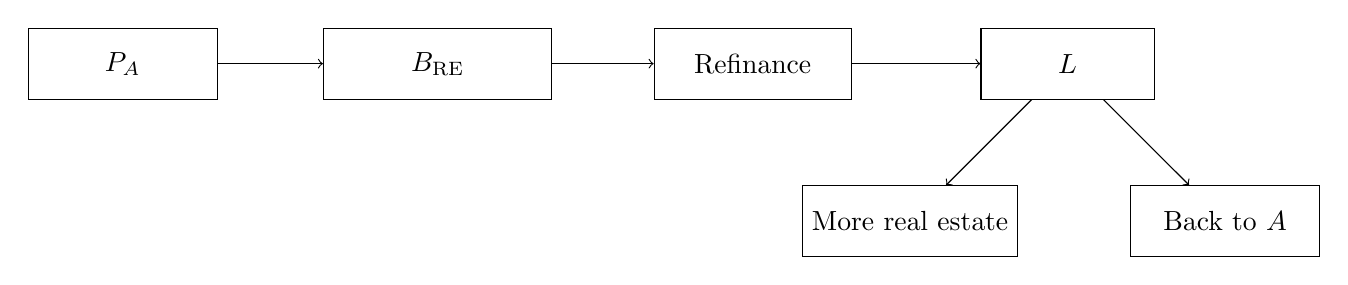
\begin{tikzpicture}[x=1cm,y=1cm]
\node[draw, rectangle, minimum width=2.4cm, minimum height=0.9cm] (a) at (0,0) {$P_A$};
\node[draw, rectangle, minimum width=2.9cm, minimum height=0.9cm] (b) at (4,0) {$B_{\mathrm{RE}}$};
\node[draw, rectangle, minimum width=2.5cm, minimum height=0.9cm] (c) at (8,0) {Refinance};
\node[draw, rectangle, minimum width=2.2cm, minimum height=0.9cm] (d) at (12,0) {$L$};
\node[draw, rectangle, minimum width=2.6cm, minimum height=0.9cm] (e) at (10,-2) {More real estate};
\node[draw, rectangle, minimum width=2.4cm, minimum height=0.9cm] (f) at (14,-2) {Back to $A$};

\draw[->] (a) -- (b);
\draw[->] (b) -- (c);
\draw[->] (c) -- (d);
\draw[->] (d) -- (e);
\draw[->] (d) -- (f);
\end{tikzpicture}
\end{figure}

The lecture's intended logic is the following:
\begin{enumerate}
\item Business \(A\) throws off profit.
\item That profit is moved into real estate \(B_{\mathrm{RE}}\).
\item Real estate is refinanced.
\item Refinancing creates liquidity \(L\) without, in the interviewee's description, being taxed like ordinary realized income.
\item The newly available cash is recycled into more business or more property.
\end{enumerate}

The speaker then adds a cautionary counterexample from his own life. He says he bought his first properties in cash, bootstrapped his business in cash, and later discovered that heavy cash purchase behavior had left him without the credit profile needed to obtain a mortgage, even when he had one million dollars in cash. The lecture therefore does not simply praise prudence. It claims that refusing all leverage can itself become a constraint.

\section{AI as a Second Kind of Leverage}

The lecture then interrupts the field sequence with an AI interlude. At first this looks like a sponsor detour, but structurally it continues the same theme. In the previous section leverage meant debt and refinancing. Here leverage means drafting speed, tone control, and response prediction.

The host's point is not that AI replaces a person. It is that AI increases throughput in ordinary business communication: pitches, proposals, outreach, revision, and clarification. The lecture treats language as an operating surface. Faster, clearer, more strategically phrased communication is itself a business multiplier.

So the AI section belongs in the chapter, but it should remain short. Its job is to preserve continuity in the lecture's larger thesis: wealth is built not only by brute effort, but by systems that compress time, reduce friction, and expand the output of a fixed human hour.

\section{From W2 Labor to the First Exit Step}

After the AI interlude, the lecture returns to the street and restarts one of its opening contrasts. We hear again that a person may be wealthy rather than merely rich, but now the distinction is pushed into a sharper institutional claim: the wage structure is not where durable wealth is usually formed.

The interviewee says he quit a W2 job, performed the same work on his own account, and thereby stopped making someone else rich. The lecture then asks the right next question. It does not ask for inspiration; it asks for the first actionable step.

\subsection{Question \& Answer}

What is the first actionable step out of corporate America?

The answer is not ``quit immediately.'' The answer is to reinterpret the current job as paid training. This is an epistemic claim before it is a career claim.

We may compress that learning ladder into the following form:
\begin{equation}
\text{unknown unknowns} \to \text{known unknowns} \to \text{operational competence} \to \text{independent execution}.
\end{equation}

This is one of the lecture's better pieces of advice. Many businesses fail, the speaker says, because people enter industries they do not understand. They mistake customer experience for operator knowledge. They like bowling, so they think they should own a bowling alley. They have been inside a bar, so they think they can run one. The lecture's corrective is exact: stay inside the industry long enough that you can see the inefficiencies, the wasted time, the corporate clutter, the things that could be done better. Only then does the option of independence become technically meaningful.

\paragraph{Worked cashflow example.}
The same interview then turns to what keeps people broke. Here the lecture gives us a concrete household arithmetic example. Let annual income be \(I\), annual expenditure be \(E\), and annual savings be \(S\), with
\begin{equation}
S = I - E.
\end{equation}
The lecture's numbers are
\begin{align}
I &\approx 225{,}000,\\
S &\approx -30{,}000,
\end{align}
in dollars per year. Solving for expenditure gives
\begin{equation}
E = I - S \approx 255{,}000.
\end{equation}

Let us write the derivation as a short sequence:
\begin{enumerate}
\item Take the reported annual income \(I\approx 225{,}000\).
\item Translate ``losing \(30{,}000\) each year'' into negative saving, \(S\approx -30{,}000\).
\item Use the identity \(S=I-E\).
\item Rearranging gives \(E=I-S\).
\item Hence \(E\approx 255{,}000\).
\end{enumerate}

The lecture's moral is clear. A large salary is not the same thing as wealth if the expenditure line is still larger. The numerical example is small, but it does real work: it converts a cultural complaint about keeping up with the Joneses into a balance-sheet statement.

\section{EBITDA, Margins, and the Price of a Business}

The same interview then tightens into explicit exit arithmetic. The question is not merely how to run a business, but how to sell one for tens of millions.

\subsection{Question \& Answer}

What is the trick to selling a company for tens of millions of dollars?

The answer given in the lecture is EBITDA. The interviewee immediately glosses this in rough speech as ``profit.'' We should preserve that simplification, but cautiously. At the level of the lecture, the intended point is that buyers pay for cash-generating ability, not for admiration.

Let \(\mu\) denote profit margin and let \(k\) denote the acquisition multiple. Then the lecture can be read through the standard shorthand
\begin{equation}
\mu = \frac{\text{profit}}{\text{revenue}},\qquad EV \approx k\cdot \text{EBITDA}.
\end{equation}

The striking reported numbers are
\begin{align}
\mu_{\text{speaker}} &\approx 0.83,\\
\mu_{\text{industry}} &\approx 0.22.
\end{align}

This deserves a compact calculation. The interviewee claims that, from a revenue standpoint, his company was as large as the others, but with far fewer employees. If we take that comparison at face value, then the ratio of cash-generating intensity is approximately
\begin{equation}
\frac{\mu_{\text{speaker}}}{\mu_{\text{industry}}}
\approx
\frac{0.83}{0.22}
\approx 3.77.
\end{equation}

Now assume, again only as a first reading of the lecture's logic, that comparable firms sell at comparable multiples \(k\). Then the enterprise-value ratio tracks the EBITDA ratio, and at similar revenue it tracks the margin ratio:
\begin{align}
\frac{EV_{\text{speaker}}}{EV_{\text{industry}}}
&\approx
\frac{k\cdot \text{EBITDA}_{\text{speaker}}}{k\cdot \text{EBITDA}_{\text{industry}}}\\
&\approx
\frac{\text{EBITDA}_{\text{speaker}}}{\text{EBITDA}_{\text{industry}}}\\
&\approx
\frac{\mu_{\text{speaker}}}{\mu_{\text{industry}}}
\approx 3.77.
\end{align}

This is not a universal formula for broker sales; it is a disciplined reading of the lecture's point. If top-line scale is similar, then cost structure can dominate outcome. A company that converts revenue into profit at roughly \(83\%\) instead of \(22\%\) is not a slightly better business. It is, from the buyer's standpoint, a much more valuable machine.

The host then pauses and recaps the interview: paid training, EBITDA, and the difference between rich and wealthy. That recap matters. It tells us which ideas the lecture itself wants carried forward.

\section{Recurring Revenue, Discipline, Inheritance, and Time}

The final movement of the lecture does not abandon arithmetic, but it spreads it across shorter interviews and aphoristic answers.

First comes recurring revenue. A later interviewee says he chose payments processing because he wanted residual income. The lecture does not write a recurrence relation, but the business intuition is clean: each month need not begin from zero if previously won accounts continue to throw off revenue. That is why recurring revenue is more attractive than one-off transaction volume. It changes the base from which the next period begins.

Then the lecture slows into moral arithmetic. We are told that there are two pains, discipline and regret, and that regret is heavier. We are told to ignore doubters, to continue after failure, and to learn from mistakes rather than repeat them. These claims are not presented as equations, but they do function like update rules: repeated bad reactions to the same error signal intellectual stagnation.

Inheritance enters next. One interviewee says coming from money was, for him, a handicap rather than a blessing, because it prevented him from learning what the first self-earned dollar feels like. This is a useful counterweight to simplistic desire for starting capital. Money can accelerate; it can also anesthetize.

The lecture closes by moving from finance to time. ``Live each day as if it were your last'' is not a sentimental line here. It is attached to a precise claim: time is the one asset we cannot bank. That point is then coupled to association. Who we stand beside changes the path we take. In the lecture's final cadence, wealth is not only a matter of revenue, debt, or margin; it is also a matter of social environment and the rate at which one's days are spent.

\section{Summary}

The lecture begins with a street-level distinction between rich and wealthy and then spends the rest of its time filling that distinction with mechanism. The mechanism is varied but coherent: visibility precedes trust, scale matters more than mere effort, debt can be used as leverage, a job can be treated as paid training, spending can outrun income even at high salary, and business value depends on the profit stream a buyer can multiply.

What gives the lecture its shape is not a single formula but a repeated movement from anecdote to claim to mechanism. We begin with access under friction, pass through marketing and leverage, move into ownership and exit math, and end with residual income, discipline, time, and association. In that sense the chapter's final lesson is the same as its first one: wealth is best understood not as a visible object, but as a structure extended through time.